\chapter{Theory background}
\label{ch:theory}

This chapter presents the technologies that are used in the system developed for this project, putting the emphasis on understanding the main concepts and introducing the terminology and notation required to fully understand the system itself, which is described in the next chapter. This chapter is mostly based on the book \textbf{Dive into Dive Learning (D2L)} \citep{Zhang2019d2l}, published online under a Creative Commons License (CC BY-NC-SA 4.0), with some modifications. In particular, we have excluded all the source code, rewritten some paragraphs to keep the consistence with the context, and added additional material to some parts that were of particular interest for our purposes.

This chapter will cover the following topics:

\begin{itemize}
    \item Convolutional Neural Networks (\cref{sec:cnn})
    \item Recurrent Neural Neworks (\cref{sec:rnn})
    \item Encoder-Decoder Architecture (\cref{sec:encoder-decoder})
    \item Attention Mechanism (\cref{sec:attention})
\end{itemize}

A basic understanding of neural networks is assumed, if not, the reader is referred to some introductory guide. In particular, we recommend chapters 3 and 4 of the D2L book referred above.

\section{Convolutional Neural Networks}\label{sec:cnn}

As we have seen in the encoder-decoder architecture, the encoder used for image captioning is typically a Convolutional Neural Network (CNN). In this section we provide a brief explanation of this kind of network architecture and introduce some of the most remarkable examples, of which some have been used for the system developed in this project.

\subsection{From fully connected layers to convolutions}

2012 was the first year that neural nets grew to prominence as Alex Krizhevsky used them to win that year’s ImageNet Large Scale Visual Recognition Competition (ILSVRC) competition \citep{Krizhevsky2012}, with an astounding drop of the classification error record from 26\% to 15\%. Ever since then, a host of companies have been using deep learning at the core of their services, including Facebook (face recognition), Google (photo search, translation, voice recognition), Amazon (product recommendations), Pinterest (feed personalization), and Instagram (search infrastructure), amongst others.

Classical neural networks, as the Multi-Layer Perceptron (MLP), and fully connected architectures in general, were designed to work with tabular data, that is, data consisting of rows corresponding to examples and columns corresponding to features. With tabular data, we might anticipate that pattern we seek could require modeling interactions among the features, but do not assume anything a priori about which features are related to each other or in what way. In such cases, there is no way of exploiting such interactions when designing the network architecture, and MLPs are probably the best approach. However, once we start dealing with high-dimensional perceptual data, these "structure-less" networks can grow very unwieldy. 

For instance, let’s consider the task of classifying pictures into either cats or dogs. Say that we do a thorough job in data collection, collecting an annotated set of high-quality 1-megapixel photographs. This means that the input into a network has 1 million dimensions. Even an aggressive reduction to 1,000 hidden dimensions would require a dense (fully-connected) layer to support  $10^9$  parameters. Unless we have an extremely large dataset (perhaps billions?), lots of GPUs, a talent for extreme distributed optimization, and an extraordinary amount of patience, learning the parameters of this network may turn out to be impossible.

A careful reader might object to this argument on the basis that 1 megapixel resolution may not be necessary. However, while you could get away with 100,000 pixels, we grossly underestimated the number of hidden nodes that it typically takes to learn good hidden representations of images. Learning a binary classifier with so many parameters might seem to require that we collect an enormous dataset, perhaps comparable to the number of dogs and cats on the planet. And yet both humans and computers are able to distinguish cats from dogs quite well, seemingly contradicting these conclusions. That’s because images exhibit rich structure that is typically exploited by humans and machine learning models alike. For example, when perceiving images, the are two important properties that our visual systems use:

\begin{itemize}
    \item \textit{Translation invariance}: vision should respond similarly to the same object regardless of where it appears in the image.
    \item \textit{Locality}: for certain tasks our vision should focus on local regions, without regard for what else is happening in the image at greater distances.
\end{itemize}

Convolutional Neural Networks, or \textit{ConvNets}, for short, are a kind of artificial neural networks designed specifically to benefit  from these properties of the visual system. In fact, ConvNets were inspired by biological processes in that the connectivity pattern between neurons resembles the organization of the animal visual cortex. Individual cortical neurons respond to stimuli only in a restricted region of the visual field known as the receptive field. The receptive fields of different neurons partially overlap such that they cover the entire visual field.

ConvNets get their name from a mathematical operation called \textit{convolution}, although they actually correspond to a similar operation called \textit{cross-correlation}, represented by an asterisk within a circle, $\circledast$. ConvNets are built by stacking successive layers of units that apply two types of operation: convolutions (cross-correlation) and pooling. Now let us describe how these operations work in practice.

\subsection{Convolution layers}\label{subsec:conv_layers}

\subsubsection{The Cross-correlation operation}

The most important operation performed by ConvNets is the cross-correlation operation, often called \textit{convolution} operation, which takes an input array and a \textit{correlation kernel} array, and produce an output array through a \textit{cross-correlation operation}. Images are represented as 2D arrays of pixels, plus a third dimension when color channels are considered. But for the sake of simplicity, let's start with a 2D representation of images. 

\begin{figure}[hpt]
	\centering
	\includesvg{images/ch3/correlation.svg}
	\caption{Two dimensional cross-correlation operation. The shaded portions are the first output element and the input and kernel array elements used in its computation: $0 \times 0+1 \times 1+3 \times 2+4 \times 3=19$}
	\label{fig:correlation}
\end{figure}

In the two-dimensional cross-correlation operation (\cref{fig:correlation}), we begin with the convolution window positioned at the top-left corner of the input array and slide it across the input array, both from left to right and top to bottom. When the convolution window slides to a certain position, the input subarray contained in that window and the kernel array are multiplied (element-wise) and the resulting array is summed up yielding a single scalar value. This result is precisely the value of the output array at the corresponding location. Here, the output array has a height of 2 and width of 2 and the four elements are derived from the two-dimensional cross-correlation operation:

\begin{align*}
0 \times 0+1 \times 1+3 \times 2+4 \times 3=19,\\
1 \times 0+2 \times 1+4 \times 2+5 \times 3=25,\\
3 \times 0+4 \times 1+6 \times 2+7 \times 3=37,\\
4 \times 0+5 \times 1+7 \times 2+8 \times 3=43.
\end{align*}

Note that along each axis, the output array is slightly smaller than the input. Because the kernel has a width greater than one, and we can only computer the cross-correlation for locations where the kernel fits wholly within the image, the output size is given by the input size $H \times W$  minus the size of the kernel $h \times w$ via $(H-h+1)\times(W-w+1)$. This is the case since we need enough space to \textit{shift} the kernel across the image.

A convolutional layer cross-correlates (\textit{convolves}) the input and kernels and adds a scalar bias $b$ to produce an output. The parameters of the convolutional layer are precisely the values that constitute the kernel and the scalar bias. When training the models based on convolutional layers, we typically initialize the kernels randomly, just as we would with a fully-connected layer. Optionally, a convolutional layer may also apply an activation function $g$ to produce its final output, although we will not explain it here, since it is the same as for a fully connected layer.

Correlation kernels can be seen as feature detectors; for example, they can be used to detect edges in different orientations, such as vertical lines, horizontal lines, or curves of any shape. Designing an edge detector by finite differences $[1, -1]$ is neat if we know this is precisely what we are looking for. However, as we look at larger kernels, and consider successive layers of convolutions, it might be impossible to specify precisely what each filter should be doing manually. Fortunately, we do not need to define kernels by hand, since they can be learned automatically using backpropagation, as the weights of a fully connected layer.

\begin{figure}[hpt]
	\centering
	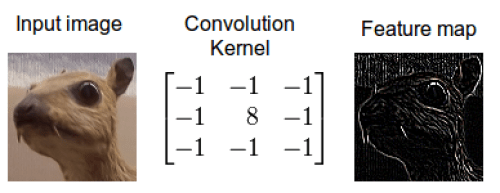
\includegraphics[scale=0.5]{images/ch3/edge-detection.png}
	\caption{Example of a convolution kernel for edge detection}
	\label{fig:edge-detection}
\end{figure}

\subsubsection{Padding}

In the previous example, our input had a height and width of 3 and a convolution kernel with a height and width of 2, yielding an output with a height and a width of 2. In general, assuming the input shape is  $n_h \times n_w$  and the convolution kernel window shape is $k_h \times k_w$, then the output shape will be

$$(n_h-k_h+1) \times (n_w-k_w+1)$$
 
Therefore, the output shape of the convolutional layer is determined by the shape of the input and the shape of the convolution kernel window.

In several cases we might want to incorporate particular techniques --padding and stride-- regarding the size of the output:
\begin{itemize}
    \item In general, since kernels generally have width and height greater than 1, that means that after applying many successive convolutions, we will wind up with an output that is much smaller than our input. If we start with a $240\times240$ pixel image, 10 layers of $5\times5$ convolutions reduce the image to $200\times200$ pixels, slicing off 30\% of the image and with it obliterating any interesting information on the boundaries of the original image. Padding handles this issue.
    \item In some cases, we want to reduce the resolution drastically if say we find our original input resolution to be unwieldy. Strides can help in these instances.
\end{itemize}

\begin{figure}[hpt]
	\centering
	\includesvg{images/ch3/conv_pad.svg}
	\caption{Two-dimensional cross-correlation with padding. The shaded portions are the input and kernel array elements used by the first output element: $0\times0+0\times1+0\times2+0\times3=0$}
	\label{fig:conv_pad}
\end{figure}

In general, if we add a total of  $p_h$  rows of padding (roughly half on top and half on bottom) and a total of  $p_w$  columns of padding (roughly half on the left and half on the right), the output shape will be

$$(n_h-k_h+p_h+1)\times(n_w-k_w+p_w+1)$$
 
This means that the height and width of the output will increase by  $p_h$  and  $p_w$  respectively.

In many cases, we will want to set  $p_h=k_h-1$  and  $p_w=k_w-1$  to give the input and output the same height and width. This will make it easier to predict the output shape of each layer when constructing the network. Assuming that  $k_h$  is odd here, we will pad  $p_h/2$ rows on both sides of the height. If $k_h$  is even, one possibility is to pad  $\lceil p_h/2\rceil$  rows on the top of the input and  $\lfloor p_h/2\rfloor$  rows on the bottom. We will pad both sides of the width in the same way.

ConvNets commonly use correlation kernels with odd height and width values, such as 1, 3, 5, or 7. Choosing odd kernel sizes has the benefit that we can preserve the spatial dimensionality while padding with the same number of rows on top and bottom, and the same number of columns on left and right.

Moreover, this practice of using odd kernels and padding to precisely preserve dimensionality offers a clerical benefit. For any two-dimensional array $X$, when the kernels size is odd and the number of padding rows and columns on all sides are the same, producing an output with the same height and width as the input, we know that the output $Y[i,j]$ is calculated by cross-correlation of the input and convolution kernel with the window centered on $X[i,j]$.

\subsubsection{Stride}

When computing the cross-correlation, we start with the convolution window at the top-left corner of the input array, and then slide it over all locations both down and to the right. In previous examples, we default to sliding one pixel at a time. However, sometimes, either for computational efficiency or because we wish to downsample, we move our window more than one pixel at a time, skipping the intermediate locations.

We refer to the number of rows and columns traversed per slide as the stride. So far, we have used strides of 1, both for height and width. Sometimes, we may want to use a larger stride. \cref{fig:conv_stride} shows a two-dimensional cross-correlation operation with a stride of 3 vertically and 2 horizontally. We can see that when the second element of the first column is output, the convolution window slides down three rows. The convolution window slides two columns to the right when the second element of the first row is output. When the convolution window slides two columns to the right on the input, there is no output because the input element cannot fill the window (unless we add padding).

\begin{figure}[hpt]
	\centering
	\includesvg{images/ch3/conv_stride.svg}
	\caption{Cross-correlation with strides of 3 and 2 for height and width respectively. The shaded portions are the output element and the input and core array elements used in its computation: $0\times0+0\times1+1\times2+2\times3=8,  0\times0+6\times1+0\times2+0\times3=6$}
	\label{fig:conv_stride}
\end{figure}

In general, when the stride for the height is $s_h$  and the stride for the width is $s_w$ , the output shape is

$$\lfloor(n_h-k_h+p_h+s_h)/s_h\rfloor \times \lfloor(n_w-k_w+p_w+s_w)/s_w\rfloor$$
 
If we set $p_h=k_h-1$  and  $p_w=k_w-1$ , then the output shape will be simplified to $\lfloor(n_h+s_h-1)/s_h\rfloor \times \lfloor(n_w+s_w-1)/s_w\rfloor$. Going a step further, if the input height and width are divisible by the strides on the height and width, then the output shape will be $(n_h/s_h)\times(n_w/s_w)$.

For the sake of brevity, when the padding number on both sides of the input height and width are $p_h$  and $p_w$  respectively, we call the padding $(p_h,p_w)$. Specifically, when  $p_h=p_w=p$, the padding is $p$. When the strides on the height and width are $s_h$ and $s_w$, respectively, we call the stride $(s_h,s_w)$. Specifically, when $s_h=s_w=s$, the stride is $s$. By default, the padding is 0 and the stride is 1. In practice we rarely use inhomogeneous strides or padding, i.e., we usually have $p_h=p_w$ and $s_h=s_w$.

\subsubsection{Multiple Input and Output Channels}

While we have described the multiple channels that comprise each image (e.g. color images have the standard RGB channels to indicate the amount of red, green and blue), until now, we simplified all of our numerical examples by working with just a single input and a single output channel. This has allowed us to think of our inputs, convolutional kernels, and outputs each as two-dimensional arrays.

When we add channels into the mix, our inputs and hidden representations both become three-dimensional arrays. For example, each RGB input image has shape $3\times h\times w$. We refer to this axis, with a size of 3, as the channel dimension. In this section, we will take a deeper look at convolution kernels with multiple input and multiple output channels.

\subsubsubsection{Multiple Input Channels}

When the input data contains multiple channels, we need to construct a convolution kernel with the same number of input channels as the input data, so that it can perform cross-correlation with the input data. Assuming that the number of channels for the input data is $c_i$, the number of input channels of the convolution kernel also needs to be $c_i$. If our convolution kernel’s window shape is $k_h\times k_w$, then when $c_i=1$, we can think of our convolution kernel as just a two-dimensional array of shape $k_h\times k_w$.

However, when $c_i>1$, we need a kernel that contains an array of shape $k_h\times k_w$ for each input channel. Concatenating these $c_i$ arrays together yields a convolution kernel of shape $c_i\times k_h\times k_w$. Since the input and convolution kernel each have $c_i$ channels, we can perform a cross-correlation operation on the two-dimensional array of the input and the two-dimensional kernel array of the convolution kernel for each channel, adding the $c_i$ results together (summing over the channels) to yield a two-dimensional array. This is the result of a two-dimensional cross-correlation between multi-channel input data and a multi-input channel convolution kernel.

\cref{fig:conv_multi_in} shows an example of a 2D cross-correlation with two input channels. 

\begin{figure}[hpt]
	\centering
	\includesvg{images/ch3/conv_multi_in.svg}
	\caption{Cross-correlation computation with 2 input channels. The shaded portions are the first output element as well as the input and kernel array elements used in its computation:  $(1 \times 1+2 \times 2+4\times3+5\times4)+(0\times0+1 \times 1+3\times2+4\times3)=56.$}
	\label{fig:conv_multi_in}
\end{figure}

\subsubsubsection{Multiple Output Channels}

Regardless of the number of input channels, so far we always ended up with one output channel. However, as we discussed earlier, it turns out to be essential to have multiple channels at each layer. In the most popular neural network architectures, we actually increase the channel dimension as we go higher up in the neural network, typically downsampling to trade off spatial resolution for greater channel depth. Intuitively, you could think of each channel as responding to some different set of features. Reality is a bit more complicated than the most naive intepretations of this intuition since representations are not learned independently but are rather optimized to be jointly useful. So it may not be that a single channel learns an edge detector but rather that some direction in channel space corresponds to detecting edges.

Denote by $c_i$ and $c_o$  the number of input and output channels, respectively, and let $k_h$ and $k_w$ be the height and width of the kernel. To get an output with multiple channels, we can create a kernel array of shape $c_i \times k_h \times k_w$ for each output channel. We concatenate them on the output channel dimension, so that the shape of the convolution kernel is $c_o \times c_i \times k_h \times k_w$. In cross-correlation operations, the result on each output channel is calculated from the convolution kernel corresponding to that output channel and takes input from all channels in the input array.

\subsubsubsection{1 x 1 convolutional layers}

At first, a $1 \times 1$  convolution, i.e.  $k_h=k_w=1$, does not seem to make much sense. After all, a convolution correlates adjacent pixels. A $1 \times 1$ convolution obviously does not. Nonetheless, they are popular operations that are sometimes included in the designs of complex deep networks. Let’s see in some detail what it actually does.

Because the minimum window is used, the $1 \times 1$ convolution loses the ability of larger convolutional layers to recognize patterns consisting of interactions among adjacent elements in the height and width dimensions. The only computation of the $1 \times 1$ convolution occurs on the channel dimension.

\cref{fig:conv_1x1} shows the cross-correlation computation using the $1 \times 1$ convolution kernel with 3 input channels and 2 output channels. Note that the inputs and outputs have the same height and width. Each element in the output is derived from a linear combination of elements at the same position in the input image. You could think of the $1 \times 1$  convolutional layer as constituting a fully-connected layer applied at every single pixel location to transform the $c_i$ corresponding input values into $c_o$ output values. Because this is still a convolutional layer, the weights are tied across pixel location Thus the $1 \times 1$  convolutional layer requires $c_o \times c_i$ weights (plus the bias terms).

\begin{figure}[hpt]
	\centering
	\includesvg{images/ch3/conv_1x1.svg}
	\caption{Cross-correlation computation using a $1 \times 1$ convolution kernel with 3 input channels and 2 output channels. The inputs and outputs have the same height and width.}
	\label{fig:conv_1x1}
\end{figure}

\subsection{Pooling layers}\label{subsec:pool_layers}

Often, as we process images, we want to gradually reduce the spatial resolution of our hidden representations, aggregating information so that the higher up we go in the network, the larger the receptive field (in the input) to which each hidden node is sensitive.

Often our ultimate task asks some global question about the image, e.g., does it contain a cat? So typically the nodes of our final layer should be sensitive to the entire input. By gradually aggregating information, yielding coarser and coarser maps, we accomplish this goal of ultimately learning a global representation, while keeping all of the advantages of convolutional layers at the intermediate layers of processing.

Moreover, when detecting lower-level features, such as edges, we often want our representations to be somewhat invariant to translation. For instance, if we take the image $X$ with a sharp delineation between black and white and shift the whole image by one pixel to the right, i.e. $Z[i,j] = X[i,j+1]$ then the output for the new image $Z$ might be vastly different. The edge will have shifted by one pixel and with it all the activations. In reality, objects hardly ever occur exactly at the same place. In fact, even with a tripod and a stationary object, vibration of the camera due to the movement of the shutter might shift everything by a pixel or so.

Pooling layers serve the dual purpose of mitigating the sensitivity of convolutional layers to location and of spatially downsampling representations.

\subsubsection{Maximum Pooling and Average Pooling}

Like convolutional layers, pooling layers apply a fixed-shape window that slides over all regions in the input according to its stride, computing a single output for each location traversed by the fixed-shape window (sometimes known as the pooling window). However, unlike convolutional layers, which need parameters to represent the correlation kernels, the pooling layer contains no parameters (there is no kernel). Instead, pooling operators are deterministic, typically calculating either the maximum or the average value of the elements in the pooling window. These operations are called maximum pooling (\textit{max pooling} for short) and \textit{average pooling}, respectively.

In both cases, as with the cross-correlation operator, we can think of the pooling window as starting from the top left of the input array and sliding across the input array from left to right and top to bottom. At each location that the pooling window hits, it computes the maximum or average value of the input subarray in the window (depending on whether max or average pooling is employed).

\begin{figure}[hpt]
	\centering
	\includesvg{images/ch3/pooling.svg}
	\caption{Maximum pooling with a pooling window shape of $2\times2$. The shaded portions represent the first output element and the input element used for its computation:  $\max(0,1,3,4)=4$.}
	\label{fig:pooling}
\end{figure}

The output array in \cref{fig:pooling} has a height of 2 and a width of 2. The four elements are derived from the maximum value of $\text{max}$:

\begin{align*}
\max(0,1,3,4)=4,\\
\max(1,2,4,5)=5,\\
\max(3,4,6,7)=7,\\
\max(4,5,7,8)=8.\\
\end{align*}

A pooling layer with a pooling window shape of $p \times q$ is called a $p \times q$ pooling layer. The pooling operation is called $p \times q$ pooling.

Let us return to the object edge detection example mentioned at the beginning of this section. Now we will use the output of the convolutional layer as the input for $2 \times 2$  max pooling. Set the convolutional layer input as $X$ and the pooling layer output as $Y$. Whether or not the values of $X[i, j]$ and $X[i, j+1]$ are different, or $X[i, j+1]$ and $X[i, j+2]$ are different, the pooling layer outputs all include $Y[i, j]=1$. That is to say, using the $2 \times 2$ maximum pooling layer, we can still detect if the pattern recognized by the convolutional layer moves no more than one element in height and width.

\subsubsection{Padding and Stride}

As with convolutional layers, pooling layers can also change the output shape. And as before, we can alter the operation to achieve a desired output shape by padding the input and adjusting the stride.

When processing multi-channel input data, the pooling layer pools each input channel separately, rather than adding the inputs of each channel by channel as in a convolutional layer. This means that the number of output channels for the pooling layer is the same as the number of input channels

\subsubsection{Batch normalization}\label{subsubsec:batch-norm}

Training deep models is difficult and getting them to converge in a reasonable amount of time can be tricky. In this section, we describe batch normalization, one popular and effective technique that has been found to accelerate the convergence of deep nets and together with residual blocks, which we cover later has recently enabled practitioners  to routinely train networks with over 100 layers.

Let's review some of the practical challenges when training deep networks.

\begin{enumerate}
    \item Data preprocessing often proves to be a crucial consideration for effective statistical modeling. Standardizing input data typically makes it easier to train models since parameters are a-priori at a similar scale.
    \item For a typical MLP or CNN, as we train the model, the activations in intermediate layers of the network may assume different orders of magnitude (both across nodes in the same layer, and over time due to updating the model's parameters). The authors of the batch normalization technique postulated that this drift in the distribution of activations could hamper the convergence of the network. Intuitively, we might conjecture that if one layer has activation values that are 100x that of another layer, we might need to adjust learning rates adaptively per layer (or even per node within a layer).
    \item Deeper networks are complex and easily capable of overfitting. This means that regularization becomes more critical. Empirically, we note that even with dropout, models can overfit badly and we might benefit from other regularization heuristics.
\end{enumerate}

In 2015, \cite{Ioffe2015} introduced Batch Normalization (BN), a clever heuristic that has proved immensely useful for improving the reliability and speed of convergence when training deep models. In each training iteration, BN normalizes the activations of each hidden layer node (on each layer where it is applied) by subtracting its mean and dividing by its standard deviation, estimating both based on the current minibatch. Note that if our batch size was $1$,  we wouldn't be able to learn anything because during training, every hidden node would take value $0$. However, with large enough minibatches, the approach proves effective and stable.

In a nutshell, the idea in Batch Normalization is  to transform the activation at a given layer from $\mathbf{x}$ to

$$\mathrm{BN}(\mathbf{x}) = \mathbf{\gamma} \odot \frac{\mathbf{x} - \hat{\mathbf{\mu}}}{\hat\sigma} + \mathbf{\beta}$$

Here, $\hat{\mathbf{\mu}}$ is the estimate of the mean and $\hat{\mathbf{\sigma}}$ is the estimate of the variance. 
The result is that the activations are approximately rescaled to zero mean and unit variance. Since this may not be quite what we want, we allow for a coordinate-wise scaling coefficient $\mathbf{\gamma}$ and an offset $\mathbf{\beta}$. Consequently, the activations for intermediate layers cannot diverge any longer: we are actively rescaling them back to a given order of magnitude via $\mathbf{\mu}$ and $\sigma$. Intuitively, it is hoped that this normalization allows us to be more aggressive in picking large learning rates. To address the fact that in some cases the activations may actually \textit{need} to differ from standardized data, BN also introduces scaling coefficients $\mathbf{\gamma}$ and an offset $\mathbf{\beta}$.

In principle, we might want to use all of our training data to estimate the mean and variance. However, the activations corresponding to each example change each time we update our model. To remedy this problem, BN uses only the current minibatch for estimating $\hat{\mathbf{\mu}}$ and $\hat\sigma$. It is precisely due to this fact that we normalize based only on the \textit{current batch}
that \textit{batch normalization} derives its name. To indicate which minibatch $\mathcal{B}$ we draw this from, we denote the quantities with $\hat{\mathbf{\mu}}_\mathcal{B}$ and $\hat\sigma_\mathcal{B}$.

$$\hat{\mathbf{\mu}}_\mathcal{B} \leftarrow \frac{1}{|\mathcal{B}|} \sum_{\mathbf{x} \in \mathcal{B}} \mathbf{x}
\text{ and }
\hat{\mathbf{\sigma}}_\mathcal{B}^2 \leftarrow \frac{1}{|\mathcal{B}|} \sum_{\mathbf{x} \in \mathcal{B}} (\mathbf{x} - \mathbf{\mu}_{\mathcal{B}})^2 + \epsilon$$

Note that we add a small constant $\epsilon > 0$ to the variance estimate to ensure that we never end up dividing by zero, 
even in cases where the empirical variance estimate might vanish by accident. The estimates $\hat{\mathbf{\mu}}_\mathcal{B}$ 
and $\hat{\mathbf{\sigma}}_\mathcal{B}$ counteract the scaling issue by using unbiased but noisy estimates of mean and variance. 
Normally we would consider this a problem. After all, each minibatch has different data, different labels and with it, different activations, predictions and errors. As it turns out, this is actually beneficial. This natural variation appears to act as a form of regularization, conferring benefits (as observed empirically) in mitigating overfitting. 

In other recent preliminary research, \citet{Teye2018} and \citet{Luo2019} relate the properties of BN to Bayesian Priors and penalties respectively. 
In particular, this sheds some light on the puzzle why BN works best for moderate sizes of minibatches in the range 50-100.

We are now ready to take a look at how batch normalization works in practice.

\paragraph{Batch Normalization Layers}

The batch normalization methods for fully-connected layers and convolutional layers are slightly different. This is due to the dimensionality of the data 
generated by convolutional layers. We discuss both cases below. Note that one of the key differences between BN and other layers is that BN operates on a a full minibatch at a time (otherwise it cannot compute the mean and variance parameters per batch).

\paragraph{Fully-Connected Layers}

Usually we apply the batch normalization layer between the affine transformation and the activation function in a fully-connected layer. In the following, we denote by $\mathbf{u}$ the input and by $\mathbf{x} = \mathbf{W}\mathbf{u} + \mathbf{b}$ the output of the linear transform. This yields the following variant of BN:

$$\mathbf{y} = \phi(\mathrm{BN}(\mathbf{x})) =  \phi(\mathrm{BN}(\mathbf{W}\mathbf{u} + \mathbf{b}))$$

Recall that mean and variance are computed on the \textit{same} minibatch $\mathcal{B}$ on which the transformation is applied. Also recall that the scaling coefficient $\mathbf{\gamma}$ and the offset $\mathbf{\beta}$ are parameters that need to be learned. They ensure that the effect of batch normalization can be neutralized as needed.

\paragraph{Convolutional Layers}

For convolutional layers, batch normalization occurs after the convolution computation and before the application of the activation function. 
If the convolution computation outputs multiple channels, we need to carry out batch normalization for \textit{each} of the outputs of these channels, 
and each channel has an independent scale parameter and shift parameter, both of which are scalars. Assume that there are $m$ examples in the mini-batch. 
On a single channel, we assume that the height and width of the convolution computation output are $p$ and $q$, respectively. We need to carry out batch normalization for $m \times p \times q$ elements in this channel simultaneously. While carrying out the standardization computation for these elements, 
we use the same mean and variance. In other words, we use the means and variances of the $m \times p \times q$ elements in this channel rather than one per pixel.

\paragraph{Batch Normalization During Prediction}

At prediction time, we might not have the luxury of computing offsets per batch—we might be required to make one prediction at a time. Secondly, the uncertainty in $\mathbf{\mu}$ and $\mathbf{\sigma}$, as arising from a minibatch are undesirable once we've trained the model. One way to mitigate this is to compute more stable estimates on a larger set for once (e.g. via a moving average) and then fix them at prediction time. Consequently, BN behaves differently during training and at test time (recall that dropout also behaves differently at train and test times).

\subsection{Examples of concrete CNN architectures}

\subsubsection{Classical convolutional networks: LeNet}

In this section, we will introduce one of the first published convolutional neural networks whose benefit was first demonstrated by  \citet{Lecun1998}, for the purpose of recognizing handwritten digits in images. In the 90s, their experiments with \href{http://yann.lecun.com/exdb/lenet/}{LeNet} gave the first compelling evidence that it was possible to train convolutional neural networks by backpropagation. Their model achieved outstanding results at the time (only matched by Support Vector Machines at the time) and was adopted to recognize digits for processing deposits in ATM machines. Some ATMs still runn the code that Yann and his colleague Leon Bottou wrote in the 1990s.

In a rough sense, we can think LeNet as consisting of two parts: (i) a block of convolutional layers; and (ii) a block of fully-connected layers. Before getting into the weeds, let’s briefly review the model in \cref{fig:lenet}

\begin{figure}[hpt]
	\centering
	\includesvg[scale=0.4]{images/ch3/lenet.svg}
	\caption{Data flow in LeNet 5. The input is a handwritten digit, the output a probabilitiy over 10 possible outcomes.}
	\label{fig:lenet}
\end{figure}

The basic units in the convolutional block are a convolutional layer and a subsequent average pooling layer (note that max-pooling works better, but it had not been invented in the 90s yet). The convolutional layer is used to recognize the spatial patterns in the image, such as lines and the parts of objects, and the subsequent average pooling layer is used to reduce the dimensionality. The convolutional layer block is composed of repeated stacks of these two basic units. Each convolutional layer uses a $5 \times 5$  kernel and processes each output with a \textit{sigmoid} activation function (again, note that \textit{ReLU}s are now known to work more reliably, but had not been invented yet). The first convolutional layer has 6 output channels, and second convolutional layer increases channel depth further to 16.

However, coinciding with this increase in the number of channels, the height and width are shrunk considerably. Therefore, increasing the number of output channels makes the parameter sizes of the two convolutional layers similar. The two average pooling layers are of size  $2 \times 2$  and take stride 2 (note that this means they are non-overlapping). In other words, the pooling layer downsamples the representation to be precisely one quarter the pre-pooling size.

The convolutional block emits an output with size given by $(batch size, channel, height, width)$. Before we can pass the convolutional block’s output to the fully-connected block, we must flatten each example in the mini-batch. In other words, we take this 4D input and transform it into the 2D input expected by fully-connected layers: as a reminder, the first dimension indexes the examples in the mini-batch and the second gives the flat vector representation of each example. LeNet’s fully-connected layer block has three fully-connected layers, with 120, 84, and 10 outputs, respectively. Because we are still performing classification, the 10 dimensional output layer corresponds to the number of possible output classes.

Note that the height and width of the representation at each layer throughout the convolutional block is reduced (compared to the previous layer). The convolutional layer uses a kernel with a height and width of 5, which with only  2  pixels of padding in the first convolutional layer and none in the second convolutional layer leads to reductions in both height and width by 2 and 4 pixels, respectively. Moreover each pooling layer halves the height and width. However, as we go up the stack of layers, the number of channels increases layer-over-layer from 1 in the input to 6 after the first convolutional layer and 16 after the second layer. Then, the fully-connected layer reduces dimensionality layer by layer, until emitting an output that matches the number of image classes.

\cref{fig:lenet-vert} shows a diagram of LeNet5 architecture in a compressed format, the one we will use for the rest of this section.

\begin{figure}[hpt]
	\centering
	\includesvg[scale=0.7]{images/ch3/lenet-vert.svg}
	\caption{Compressed notation for LeNet5}
	\label{fig:lenet-vert}
\end{figure}


\paragraph{Summary}

\begin{itemize}
    \item A convolutional neural network (in short, ConvNet) is a network using convolutional layers.
    \item In a ConvNet we alternate between convolutions, nonlinearities and often also pooling operations.
    \item Ultimately the resolution is reduced prior to emitting an output via one (or more) dense layers.
    \item LeNet was the first successful deployment of such a network.
\end{itemize}

\subsubsection{Modern convolutional architectures}\label{subsubsec:modern_cnn}

Although convolutional neural networks were well known in the computer vision and machine learning communities following the introduction of LeNet, they did not immediately dominate the field. Although LeNet achieved good results on early small data sets, the performance and feasibility of training convolutional networks on larger, more realistic datasets had yet to be established
In fact, for much of the intervening time between the early 1990s and the watershed results of 2012, neural networks were often surpassed by other machine learning methods, such as support vector machines.

A major breakthrough came when Alex Krizhevsky and Ilya Sutskever implemented a deep convolutional neural network that could run on GPU hardware. They realized that the computational bottlenecks in CNNs (convolutions and matrix multiplications) are all operations that could be parallelized in hardware. Using two NIVIDA GTX 580s with 3GB of memory, they implemented fast convolutions. The code \href{https://code.google.com/archive/p/cuda-convnet/}{cuda-convnet} was good enough that for several years it was the industry standard and powered the first couple years of the deep learning boom.

\subsubsubsection{AlexNet: first large-scale ConvNet}

AlexNet was introduced in 2012, named after Alex Krizhevsky, the first author of the breakthrough ImageNet classification paper \citep{Krizhevsky2012}. AlexNet, which employed an 8-layer convolutional neural network, won the ImageNet Large Scale Visual Recognition Challenge 2012 by a phenomenally large margin. This network proved, for the first time, that the features obtained by learning can transcend manually-design features, breaking the previous paradigm in computer vision. The architectures of AlexNet and LeNet are \textit{very similar}, as the diagram below illustrates. Note that we provide a slightly streamlined version of AlexNet removing some of the design quirks that were needed in 2012 to make the model fit on two small GPUs.

\begin{figure}[hpt]
	\centering
	\includesvg[scale=0.8]{images/ch3/alexnet-all.svg}
	\caption{LeNet (left) and AlexNet (right)}
	\label{fig:alexnet}
\end{figure}

The design philosophies of AlexNet and LeNet are very similar, but there are also significant differences. First, AlexNet is much deeper than the comparatively small LeNet5. AlexNet consists of eight layers: five convolutional layers, two fully-connected hidden layers, and one fully-connected output layer. Second, AlexNet used the ReLU instead of the sigmoid as its activation function.

\paragraph{Architecture}

In AlexNet's first layer, the convolution window shape is $11\times11$. Since most images in ImageNet are more than ten times higher and wider than the MNIST images, objects in ImageNet data tend to occupy more pixels. Consequently, a larger convolution window is needed to capture the object. The convolution window shape in the second layer is reduced to $5\times5$, followed by $3\times3$. In addition, after the first, second, and fifth convolutional layers, the network adds maximum pooling layers with a window shape of $3\times3$ and a stride of 2. Moreover, AlexNet has ten times more convolution channels than LeNet.

After the last convolutional layer are two fully-connected layers with 4096 outputs. These two huge fully-connected layers produce model parameters of nearly 1 GB. Due to the limited memory in early GPUs, the original AlexNet used a dual data stream design,
so that each of their two GPUs could be responsible for storing and computing only its half of the model. Fortunately, GPU memory is comparatively abundant now, so we rarely need to break up models across GPUs these days.

\paragraph{Activation functions}

Second, AlexNet changed the sigmoid activation function to a simpler ReLU activation function. On the one hand, the computation of the ReLU activation function is simpler. For example, it does not have the exponentiation operation found in the sigmoid activation function. On the other hand, the ReLU activation function makes model training easier when using different parameter initialization methods. This is because, when the output of the sigmoid activation function is very close to 0 or 1, the gradient of these regions is almost 0, so that back propagation cannot continue to update some of the model parameters. In contrast, the gradient of the ReLU activation function in the positive interval is always 1. Therefore, if the model parameters are not properly initialized, the sigmoid function may obtain a gradient of almost 0 in the positive interval, so that the model cannot be effectively trained.

\paragraph{Capacity Control and Preprocessing}

AlexNet controls the model complexity of the fully-connected layer by dropout, while LeNet only uses weight decay. To augment the data even further, the training loop of AlexNet added a great deal of image augmentation, such as flipping, clipping, and color changes.
This makes the model more robust and the larger sample size effectively reduces overfitting.

\paragraph{Summary}

\begin{itemize}
    \item AlexNet has a similar structure to that of LeNet, but uses more convolutional layers and a larger parameter space to fit the large-scale data set ImageNet.
    \item Today AlexNet has been surpassed by much more effective architectures but it is a key step from shallow to deep networks that are used nowadays.
    \item Although it seems that there are only a few more lines in AlexNet's implementation than in LeNet, it took the academic community many years to embrace this conceptual change and take advantage of its excellent experimental results. This was also due to the lack of efficient computational tools.
    \item Dropout, ReLU and preprocessing were the other key steps in achieving excellent performance in computer vision tasks.
\end{itemize}

\subsubsubsection{VGG: network architecture based on repeating blocks}\label{cnn:vgg}

While AlexNet proved that deep convolutional neural networks can achieve good results, it didn't offer a general template to guide subsequent researchers in designing new networks.  In the following sections, we will introduce several heuristic concepts commonly used to design deep networks.

Progress in this field mirrors that in chip design where engineers went from placing transistors to logical elements to logic blocks. Similarly, the design of neural network architectures  had grown progressively more abstract, with researchers moving from thinking in terms of individual neurons to whole layers, and now to blocks, repeating patterns of layers.

The idea of using blocks first emerged from the \href{http://www.robots.ox.ac.uk/~vgg/}{Visual Geometry Group} (VGG) at Oxford University. In their eponymously-named VGG network, It's easy to implement these repeated structures in code with any modern deep learning framework by using loops and subroutines. 

\paragraph{VGG blocks}

The basic building block of classic convolutional networks is a sequence of the following layers: (i) a convolutional layer  (with padding to maintain the resolution), (ii) a nonlinearity such as a ReLu.

One VGG block consists of a sequence of convolutional layers,  followed by a max pooling layer for spatial downsampling. In the original VGG paper \citet{Simonyan2015} employed convolutions with $3\times3$ kernels and $2 \times 2$ max pooling with stride of $2$ (halving the resolution after each block).

\paragraph{VGG network}

Like AlexNet and LeNet, the VGG Network can be partitioned into two parts: the first consisting mostly of convolutional and pooling layers and a second consisting of fully-connected layers. The convolutional portion of the net connects several \textit{vgg block} modules in succession.

\begin{figure}[hpt]
	\centering
	\includesvg[scale=0.8]{images/ch3/vgg.svg}
	\caption{Designing a network from building blocks}
	\label{fig:vgg}
\end{figure}

The original VGG network had 5 convolutional blocks, among which the first two have one convolutional layer each and the latter three contain two convolutional layers each. The first block has 64 output channels and each subsequent block doubles the number of output channels, until that number reaches $512$. Since this network uses $8$ convolutional layers and $3$ fully-connected layers, it is often called VGG-11.

\paragraph{Summary}

\begin{itemize}
    \item VGG-11 constructs a network using reusable convolutional blocks. Different VGG models can be defined by the differences in the number of convolutional layers and output channels in each block.
    \item The use of blocks leads to very compact representations of the network definition. It allows for efficient design of complex networks.
    \item The authors of VGG experimented with various architectures. In particular, they found that several layers of deep and narrow convolutions (i.e. $3 \times 3$) were more effective than fewer layers of wider convolutions.
\end{itemize}

\subsubsubsection{NiN: Network in Network}\label{cnn:nin}

LeNet, AlexNet, and VGG all share a common design pattern: extract features exploiting \textit{spatial} structure via a sequence of convolutions and pooling layers and then post-process the representations via fully-connected layers. The improvements upon LeNet by AlexNet and VGG mainly lie in how these later networks widen and deepen these two modules. Alternatively, one could imagine using fully-connected layers earlier in the process. However, a careless use of dense layers might give up the spatial structure of the representation entirely, Network in Network (NiN) blocks offer an alternative. They were proposed by \citet{Lin2014nin} based on a very simple insight, --to use an MLP on the channels for each pixel separately.

\paragraph{NiN blocks}

Recall that the inputs and outputs of convolutional layers consist of four-dimensional arrays with axes corresponding to the batch, channel, height, and width. Also recall that the inputs and outputs of fully-connected layers are typically two-dimensional arrays corresponding to the batch, and features. The idea behind NiN is to apply a fully-connected layer at each pixel location (for each height and  width). If we tie the weights across each spatial location, we could think of this as a $1\times 1$ convolutional layer or as a fully-connected layer acting independently on each pixel location. Another way to view this is to think of each element in the spatial dimension (height and width) as equivalent to an example and the channel as equivalent to a feature.  below illustrates the main structural differences between NiN and AlexNet, VGG, and other networks.

\begin{figure}[hpt]
	\centering
	\includesvg[scale=0.8]{images/ch3/nin-compare.svg}
	\caption{The figure on the left shows the network structure of AlexNet and VGG, and the figure on the right shows the network structure of NiN.}
	\label{fig:nin-compare}
\end{figure}

The NiN block consists of one convolutional layer followed by two $1\times 1$ convolutional layers that act as per-pixel fully-connected layers with ReLU activations. The convolution width of the first layer is typically set by the user. The subsequent widths are fixed to $1 \times 1$.

\paragraph{NiN model}

The original NiN network was proposed shortly after AlexNet and clearly draws some inspiration. NiN uses convolutional layers with window shapes of $11\times 11$, $5\times 5$, and $3\times 3$, and the corresponding numbers of output channels are the same as in AlexNet. Each NiN block is followed by a maximum pooling layer with a stride of 2 and a window shape of $3\times 3$.

Once significant difference between NiN and AlexNet is that NiN avoids dense connections altogether. Instead, NiN uses an NiN block with a number of output channels equal to the number of label classes, followed by a \textit{global} average pooling layer, yielding a vector of \href{https://en.wikipedia.org/wiki/Logit}{logits}. One advantage of NiN's design is that it significantly reduces the number of required model parameters. However, in practice, this design sometimes requires increased model training time.

\paragraph{Summary}

\begin{itemize}
    \item NiN uses blocks consisting of a convolutional layer and multiple $1\times 1$ convolutional layer. This can be used within the convolutional stack to allow for more per-pixel nonlinearity.
    \item NiN removes the fully connected layers and replaces them with global average pooling (i.e. summing over all locations) after reducing the number of channels to the desired number of outputs (e.g. 10 for Fashion-MNIST).
    \item Removing the dense layers reduces overfitting. NiN has dramatically fewer parameters.
    \item The NiN design influenced many subsequent convolutional neural networks designs.
\end{itemize}

\subsubsubsection{GoogLeNet (aka Inception): networks with parallel concatenations}\label{cnn:googlenet}

In 2014, \citet{Szegedy2015} won the ImageNet Challenge, proposing a structure that combined the strengths of the NiN and repeated blocks paradigms. One focus of the paper was to address the question of which sized convolutional kernels are best. After all, previous popular networks employed choices as small as $1 \times 1$ and as large as $11 \times 11$. One insight in this paper was that sometimes it can be advantageous to employ a combination of variously-sized kernels. In this section, we will introduce GoogLeNet, presenting a slightly simplified version of the original model --we omit a few ad hoc features that were added to stabilize training
but are unnecessary now with better training algorithms available. 

\paragraph{Inception blocks}

The basic convolutional block in GoogLeNet is called an Inception block, likely named due to a quote from the movie Inception ("We Need To Go Deeper"), which launched a viral meme.

\begin{figure}[hpt]
	\centering
	\includesvg[scale=0.8]{images/ch3/inception.svg}
	\caption{Structure of the Inception block.}
	\label{fig:inception}
\end{figure}

As depicted in \cref{fig:inception}, the inception block consists of four parallel paths. The first three paths use convolutional layers 
with window sizes of $1\times 1$, $3\times 3$, and $5\times 5$ to extract information from different spatial sizes. The middle two paths perform a $1\times 1$ convolution on the input to reduce the number of input channels, reducing the model's complexity. 
The fourth path uses a $3\times 3$ maximum pooling layer, followed by a $1\times 1$ convolutional layer to change the number of channels. The four paths all use appropriate padding to give the input and output the same height and width. Finally, the outputs along each path are concatenated along the channel dimension and comprise the block's output. The commonly-tuned parameters of the Inception block are the number of output channels per layer.

To gain some intuition for why this network works so well, consider the combination of the filters. They explore the image in varying ranges.  This means that details at different extents can be recognized efficiently by different filters. At the same time, we can allocate different amounts of parameters for different ranges (e.g. more for short range but not ignore the long range entirely).

\paragraph{GoogLeNet model}

GoogLeNet uses a stack of a total of 9 inception blocks  and global average pooling to generate its estimates. Maximum pooling between inception blocks reduced the dimensionality.  The first part is identical to AlexNet and LeNet, the stack of blocks is inherited from VGG and the global average pooling avoids a stack of fully-connected layers at the end. The architecture is depicted in \cref{fig:inception-full}.

\begin{figure}[hpt]
	\centering
	\includesvg[scale=0.8]{images/ch3/inception-full.svg}
	\caption{Full GoogLeNet Model.}
	\label{fig:inception-full}
\end{figure}

\begin{enumerate}
    \item The first component uses a 64-channel $7 \times 7$ convolutional layer.
    \item The second component uses two convolutional layers: first, a 64-channel $1\times 1$ convolutional layer, then a $3\times 3$ convolutional layer that triples the number of channels. This corresponds to the second path in the Inception block.
    \item The third component connects two complete Inception blocks in series. The number of output channels of the first Inception block is $64+128+32+32=256$, and the ratio to the output channels of the four paths is $64:128:32:32=2:4:1:1$. The second and third paths first reduce the number of input channels to $96/192=1/2$ and $16/192=1/12$, respectively, and then connect the second convolutional layer. The number of output channels of the second Inception block is increased to $128+192+96+64=480$, and the ratio to the number of output channels per path is $128:192:96:64 = 4:6:3:2$. The second and third paths first reduce the number of input channels to $128/256=1/2$ and $32/256=1/8$, respectively.
    \item The fourth block is more complicated. It connects five Inception blocks in series, and they have $192+208+48+64=512$, $160+224+64+64=512$, $128+256+64+64=512$, $112+288+64+64=528$, and $256+320+128+128=832$ output channels, respectively. The number of channels assigned to these paths is similar to that in the third module: the second path with the $3\times 3$ convolutional layer outputs the largest number of channels, followed by the first path with only the $1\times 1$ convolutional layer, the third path with the $5\times 5$ convolutional layer, and the fourth path with the $3\times 3$ maximum pooling layer. The second and third paths will first reduce the number of channels according the ratio. These ratios are slightly different in different Inception blocks.
    \item The fifth block has two Inception blocks with $256+320+128+128=832$ and $384+384+128+128=1024$ output channels. The number of channels assigned to each path is the same as that in the third and fourth modules, but differs in specific values. It should be noted that the fifth block is followed by the output layer. This block uses the global average pooling layer to change the height and width of each channel to 1, just as in NiN. Finally, we turn the output into a two-dimensional array followed by a fully-connected layer whose number of outputs is the number of label classes.
\end{enumerate}
 
\paragraph{Summary}

\begin{itemize}
    \item The Inception block is equivalent to a subnetwork with four paths. It extracts information in parallel through convolutional layers of different window shapes and maximum pooling layers. $1 \times 1$ convolutions reduce channel dimensionality on a per-pixel level. Max-pooling reduces the resolution.
    \item GoogLeNet connects multiple well-designed Inception blocks with other layers in series. The ratio of the number of channels assigned in the Inception block is obtained through a large number of experiments on the ImageNet data set.
    \item GoogLeNet, as well as its succeeding versions, was one of the most efficient models on ImageNet, providing similar test accuracy with lower computational complexity.
\end{itemize}

\subsubsubsection{ResNet: residual networks}\label{cnn:resnet}

As we design increasingly deeper networks it becomes imperative to understand how adding layers can increase the complexity and expressiveness of the network. Even more important is the ability to design networks where adding layers makes networks strictly more expressive rather than just different. To make some progress we need a bit of theory.

\paragraph{Function Classes}

Consider $\mathcal{F}$, the class of functions that a specific network architecture (together with learning rates and other hyperparameter settings) can reach. That is, for all $f \in \mathcal{F}$ there exists some set of parameters $W$ that can be obtained through training on a suitable dataset. Let's assume that $f^*$ is the function that we really would like to find. If it's in $\mathcal{F}$, we're in good shape but typically we won't be quite so lucky. Instead, we will try to find some $f^*_\mathcal{F}$ which is our best bet within $\mathcal{F}$. For instance, we might try finding it by solving the following optimization problem:

$$f^*_\mathcal{F} := \mathop{\mathrm{argmin}}_f L(X, Y, f) \text{ subject to } f \in \mathcal{F}$$

It is only reasonable to assume that if we design a different and more powerful architecture $\mathcal{F}'$ we should arrive at a better outcome. In other words, we would expect that $f^*_{\mathcal{F}'}$ is 'better' than $f^*_{\mathcal{F}}$. However, if $\mathcal{F} \not\subseteq \mathcal{F}'$ there is no guarantee that this should even happen. In fact, $f^*_{\mathcal{F}'}$ might well be worse. This is a situation that we often encounter in practice - adding layers doesn't only make the network more expressive, it also changes it in sometimes not quite so predictable ways. The picture below illustrates this in slightly abstract terms.

\begin{figure}[hpt]
	\centering
	\includesvg[scale=0.5]{images/ch3/functionclasses.svg}
	\caption{Left: non-nested function classes. The distance may in fact increase as the complexity increases. Right: with nested function classes this does not happen.}
	\label{fig:functionclasses}
\end{figure}


Only if larger function classes contain the smaller ones are we guaranteed that increasing them strictly increases the expressive power of the network. This is the question that \cite{He2016resnet} considered when working on very deep computer vision models. At the heart of ResNet is the idea that every additional layer should contain the identity function as one of its elements. This means that if we can train the newly-added layer into an identity mapping $f(\mathbf{x}) = \mathbf{x}$, the new model will be as effective as the original model. As the new model may get a better solution to fit the training data set, the added layer might make it easier to reduce training errors. Even better, the identity function rather than the null $f(\mathbf{x}) = 0$ should be the the simplest function within a layer.

These considerations are rather profound but they led to a surprisingly simple solution, a residual block. With it, \citet{He2016resnet} won the ImageNet Visual Recognition Challenge in 2015. The design had a profound influence on how to build deep neural networks.

\paragraph{Residual Blocks}

Let us focus on a local neural network, as depicted below. Denote the input by $\mathbf{x}$. We assume that the ideal mapping we want to obtain by learning is $f(\mathbf{x})$, to be used as the input to the activation function. The portion within the dotted-line box in the left image must directly fit the mapping $f(\mathbf{x})$. This can be tricky if we don't need that particular layer and we would much rather retain the input $\mathbf{x}$. The portion within the dotted-line box in the right image now only needs to parametrize the \textit{deviation} from the identity, since we return $\mathbf{x} + f(\mathbf{x})$. In practice, the residual mapping is often easier to optimize. We only need to set $f(\mathbf{x}) = 0$. The right image in \cref{fig:residual-block} illustrates the basic Residual Block of ResNet. Similar architectures were later proposed for sequence models which we will study later.

\begin{figure}[hpt]
	\centering
	\includesvg[scale=0.8]{images/ch3/residual-block.svg}
	\caption{The difference between a regular block (left) and a residual block (right). In the latter case, we can short-circuit the convolutions.}
	\label{fig:residual-block}
\end{figure}

ResNet follows VGG's full $3\times 3$ convolutional layer design. The residual block has two $3\times 3$ convolutional layers with the same number of output channels. Each convolutional layer is followed by a batch normalization layer and a ReLU activation function. Then, we skip these two convolution operations and add the input directly before the final ReLU activation function. This kind of design requires that the output of the two convolutional layers be of the same shape as the input, so that they can be added together. If we want to change the number of channels or the the stride, we need to introduce an additional $1\times 1$ convolutional layer to transform the input into the desired shape for the addition operation. 

\begin{figure}[hpt]
	\centering
	\includesvg[scale=0.8]{images/ch3/ResNetBlock.svg}
	\caption{Left: regular ResNet block; Right: ResNet block with 1x1 convolution.}
	\label{fig:resnetblock}
\end{figure}

\paragraph{ResNet model}

The first two layers of ResNet are the same as those of the GoogLeNet we described before: the $7\times 7$ convolutional layer with 64 output channels and a stride of 2 is followed by the $3\times 3$ maximum pooling layer with a stride of 2. The difference is the batch normalization layer added after each convolutional layer in ResNet.

GoogLeNet uses four blocks made up of Inception blocks. However, ResNet uses four modules made up of residual blocks, each of which uses several residual blocks with the same number of output channels. The number of channels in the first module is the same as the number of input channels. Since a maximum pooling layer with a stride of 2 has already been used, it is not necessary to reduce the height and width. In the first residual block for each of the subsequent modules, the number of channels is doubled compared with that of the previous module, and the height and width are halved.

There are 4 convolutional layers in each module (excluding the $1\times 1$ convolutional layer). Together with the first convolutional layer and the final fully connected layer, there are 18 layers in total. Therefore, this model is commonly known as ResNet-18. By configuring different numbers of channels and residual blocks in the module, we can create different ResNet models, such as the deeper 152-layer ResNet-152. Although the main architecture of ResNet is similar to that of GoogLeNet, ResNet's structure is simpler and easier to modify. All these factors have resulted in the rapid and widespread use of ResNet. Below is a diagram of the full ResNet-18.

\paragraph{Summary}

\begin{itemize}
    \item Residual blocks allow for a parametrization relative to the identity function $f(\mathbf{x}) = \mathbf{x}$.
    \item Adding residual blocks increases the function complexity in a well-defined manner.
    \item We can train an effective deep neural network by having residual blocks pass through cross-layer data channels.
    \item ResNet had a major influence on the design of subsequent deep neural networks, both for convolutional and sequential nature.
\end{itemize}
 